% !TeX spellcheck = en_US

\chapter{Background}
\label{sec:background}

\section{BESSY II}

\subsection{General presentation}
BESSY II (\textbf{B}erliner \textbf{E}lektronen\-\textbf{S}peicherring-Gesellschaft für \textbf{Sy}n\-chro\-tron\-strahlung m.b.H.) is Berlin electron storage ring, aimed at producing high energy light ray by synchrotron radiation. It emits extremely brillant photons pulse ranging from the long wave terahertz region to hard X rays, with an emphasis on the soft X-ray range~\cite{web:bessy_homepage}. Scientific projects can freely apply to an experimental station, where they are able to adjust the wavelength, polarization and photon energy. More than 2000 scientists per year are using BESSY II equipment.

The storage ring has a circumference of 240~meters and provides around 50 beamlines (paths of light rays between the accelerator and experimental stations). The electrons are accelerated to an energy up to 1.7~GeV.

BESSY II was inaugurated in 1998 and is since 2009 a facility of the \textit{Helmholtz-Zentrum Berlin für Materialien und Energie} (HZB), to study material structures and processes by guest scientists.

Additionally to the guest scientists, experts and operators\todo{I don't know how to call them} ensure the good functioning of the whole facility and work on refining the quality and the stability of the light rays. 

\subsection{General functioning}
The way BESSY II functions is based on the synchrotron radiation phenomenon: any accelerated particle emits radiations (in the form of photons), with a maximal amplitude in the case of a circular acceleration. \todo{Should I detail the equations?} It can be shown~\cite{book:wille} that the radiated power in circular acceleration can be given as 
\begin{equation}
P_s = \frac{e^2 c}{6 \pi \epsilon_0}\frac{1}{(m_0 c^2)^4}\frac{E^4}{R^2}.
\end{equation}
where $c$ is the speed of light, $m_0$ the rest mass (independent of the velocity) of the particle, $e$ its charge, $E$ it's energy, $R$ the bending radius and $\epsilon_0$ the  vacuum permittivity.

Considering their low mass, the electrons are very good candidates to produce high energy radiation.

The most important properties of the synchrotron radiation are its brilliance and brightness. \todo{define...} The brightness is defined as [...] and the brilliance as [...]

The main purpose of BESSY II is to provide a light radiation with stable brilliance and brightness over time. To achieve this, the light source itself must be very stable as well. Therefore a significant attention is drawn to the control of the storage ring.

\begin{sidewaysfigure}
    \centering
    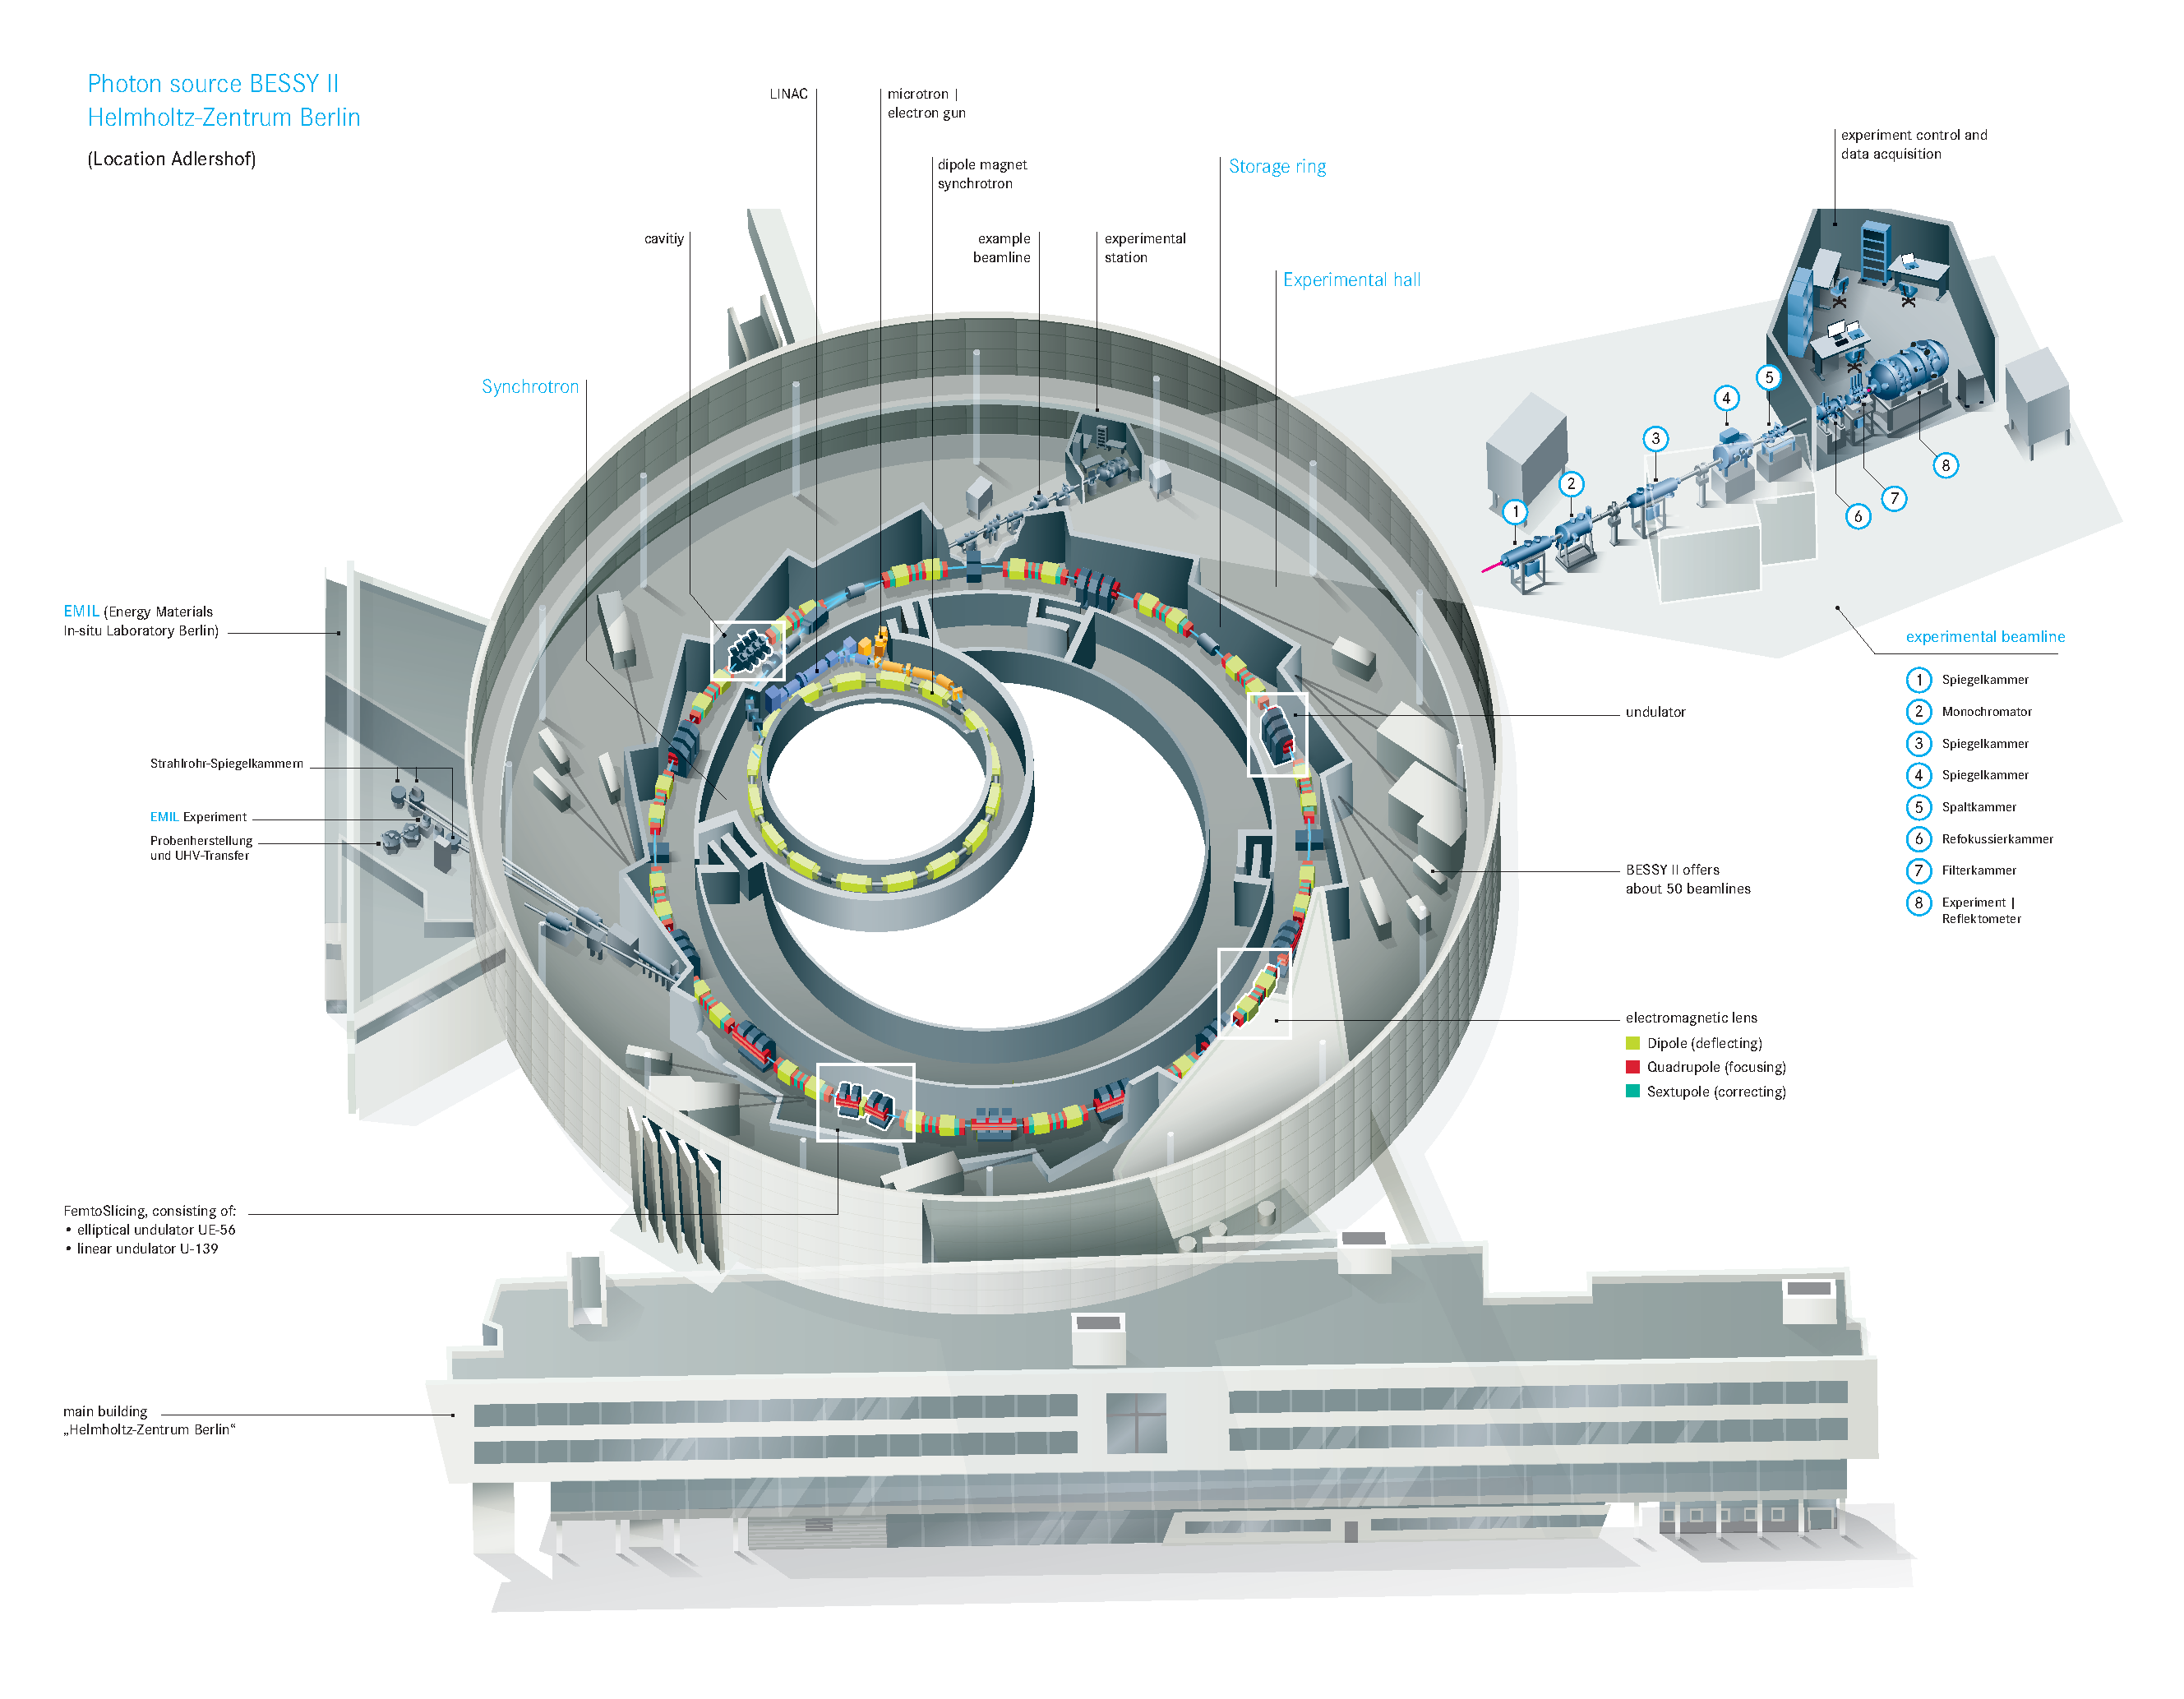
\includegraphics[width=0.8\textwidth,height=0.8\textheight,keepaspectratio]{img/bessy_acc_web.pdf}
    \caption[Bessy II facility]{\label{fig:bessy_acc_web} Bessy II facility (Source:~\cite{web:bessy_homepage})}
\end{sidewaysfigure}

In order to reach an energy of 1.7~GeV, the electrons undergo several chained accelerations (see \autoref{fig:bessy_acc_web}), namely:\todo{energies}
\begin{enumerate}
    \item an electron canon gives the electrons their first impulse
    \item a microtron accelerate them to an energy of XXX
    \item a LINAC (\textbf{lin}ear \textbf{ac}celerator) increase the energy to XXX
    \item the booster (a synchrotron) give them the final energy of XXX.
\end{enumerate}

When this energy is reached, the electrons are injected to the storage ring, which ensure that the electrons are kept at the same energy.

Because of the synchrotron radiation, the bunches of particles lose regularly their energy; therefore a new injections from the accelerations chain take place every XXX\todo{time} to repopulate the storage ring and stabilize its energy.

\section{Focus on the booster and the storage ring}
Both the booster and the storage ring are synchrotrons. The former aims at accelerating the particles, whereas the latter aims at storing them with a constant energy.

\subsection{Booster -- Synchrotron basics}
\todo[inline]{General physics of the synchrotron}

\subsection{Storage ring}
\todo[inline]{What is particular in storage ring}

\section{Orbit and distortions}
\todo[inline]{Physics + examples = 1/2 - 1 pges}

The accelerators are designed so that the particles follow a given path, which is defined in the case of synchrotrons by the successive bendings involved by the magnets. As the precision of the positioning of the magnets is limited, some errors may destabilize the orbit and increase the dispersion of the particles around the theoretical orbit. In addition, the environment produces perturbations: for instance the 50~Hz of the main power, some not perfectly isolated magnetic sources.

In order not to lose electrons in the walls of the vacuum chamber but also to increase the brightness of the synchrotron radiations (and therefore to have focused electron beams), all these residual misalignment and magnetic field errors must be corrected.


